\chapter{The Automatic Retrieval system}

This chapter aims at explaining how the text processing system was created and how it manages to extract relevant information from text like activities, locations, objects and so on.



\section{Text Processing and Word Extraction}

In the text processing stage, the query topics are analysed using Natural Language Processing tools to extract relevant words in order to retrieve the desired moment. Those words are compared with the visual concepts words obtained in the image processing stage. The text is therefore processed using a pre-trained state-of-the-art word2vec model in order to produce word embeddings.

The SpaCy library is used to analyse the query topics fully, extracting relevant words from the title, the description and narrative. The words extracted are divided into 10 categories being them : "relevant things", "activities", "dates", "locations", "inside", "outside", "negative relevant things", "negative activities", "negative locations" and "negative dates".

In order to assign words to each category some linguistic rules were defined,
such as semantic and syntactic rules. Semantic rules build the meaning of the
sentence from its words and how words combine syntactically. Syntax rules refer to
the rules that govern the ways in which words combine to form phrases, and
sentences. 

\begin{figure}[H]
    \centering
    \captionsetup{justification=centering}
    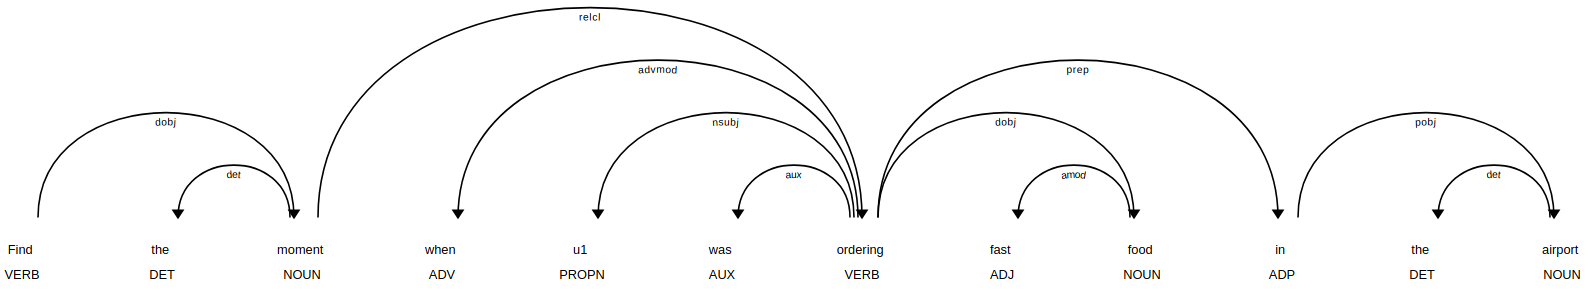
\includegraphics[width = 0.9 \textwidth]{Sections/6textprocessing/images/spacy.png}
    \caption{Linguistic annotations generated by SpaCy library for the narrative of the topic 6 of the test topics.}
    \label{fig:spacy_labels}
  \end{figure}
  
  
  
  As an example, some of the rules that were applied in the extraction of words to different categories:
  
  \begin{itemize}
      \item  If the word is a "VERB" and ends with "ing", like "ordering" then it probably is an activity and if the words that follows are "NOUN" with or without "ADJ" (adjectives) then those words are probably either a location or an object.
      \item  If the word is and "ADP" and its either "in" or "at" then the words that follow are probably locations and usually means that the moment occurs inside a location and not outside, the category "inside" is then flagged to "True" and "outside" is flagged to "False".
      \item If the word is a "NUM" (number) then it probably refers to a year.
      \item if the sentence has an auxiliary verb, the main verb usually corresponds to an activity and the words that follow the main verb may be objects or locations.
      \item If the word is an "ADJ" (adjective) then the following word is probably an object. It can also be a bi-gram like "ice cream" or in this case "fast food".
      \item If the sentence ends with "not considered relevant" the extracted words go to the negative categories.
      \item Rules for the extraction of dates, like day of the week, months, years, were also created, but do the the syntax of the test topics they were discarded in order to save time, however, for the dev topics they were used and produced good results. As an example if in the topic it was said that the moment happened on a "wednesday" or in year 2014, only pictures from wednesday or the year 2014 were retrieved.

    \end{itemize}


Using figure \ref{fig:spacy_labels} as an example, the extracted words for the different categories for the topic narrative of topic 6 from the test topics were as follows:

    \begin{itemize}
        \item \textbf{relevant things} : "fast food".
        \item \textbf{activities} : "ordering", "ordering fast food".
        \item \textbf{locations} : "airport".
        \item \textbf{inside} : "True".
        \item \textbf{outside}: "False".
       
    \end{itemize}


\section{Retrieval}

    In the retrieval step the images are recovered according to the desired query topic.
    As an example figure \ref{fig:testtopic} represents the test topic number 7.
   
    \begin{figure}[H]
        \centering
        \captionsetup{justification=centering}
        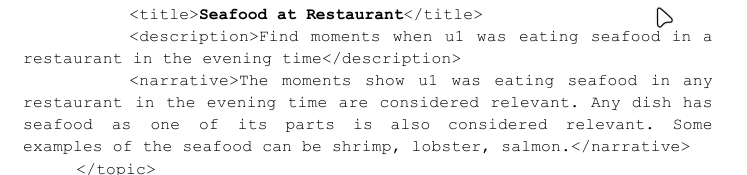
\includegraphics[width = \textwidth]{Sections/6textprocessing/images/topic.png}
        \caption{Test topic number 7.}
        \label{fig:testtopic}
      \end{figure}
      
      The extracted words of the title, description and narrative are as follows:

      \begin{itemize}
        \item \textbf{relevant things} : 
            "seafood",
            "parts",
            "shrimp",
            "lobster",
            "salmon".
        \item \textbf{activities} : "eating",
        "eating seafood"
        \item \textbf{locations} : "restaurant",  "evening time".
        \item \textbf{inside} : "True".
        \item \textbf{outside}: "False".
        \item \textbf{dates}: NULL.
        \item \textbf{negative relevant thing}: NULL.
        \item \textbf{negative activities}: NULL.
        \item \textbf{negative locations}:  NULL.
        \item \textbf{negative dates}: NULL.
       
    \end{itemize}

    The words "evening time" went to the locations category wrongly because of the previously described rule, where if a word is an "ADP" and it is "in" then the following "NOUN" is probably a location, which in this case is not correct.


    A comparison is made between the visual concept words extracted from the images and the words extracted from the topic. In order to do this, the SpaCy en\_core\_web\_md model was used, which is an english mult-task CNN trained on OntoNotes, with GloVe vectors trained on Common Crawl. This model allows for the computation of the similarity between words.

    For example the word "television" and "seafood" have a similarity of 0.0705759162558067 while "television" and "screen" have a similarity of 0.4271196001925812.

    Afterwards, a confidence score is computed for each image in the dataset for every single topic, which means that a confidence score was calculated for 2.000.000 images, which took a lot of computer processing time and resources, and made it extremely difficult to make adjustments and correct errors.

    The score is obtained through the comparison of the extracted words from the
    topic and the extracted labels from the images. The 10 pictures with the highest confidence score for each topic are retrieved.

    \section{Run 1 and Run 2 }
    Using figure \ref{fig:image_fully_processed}, the comparisons made are the following :

    \begin{itemize}
        \item The category "concepts" is compared to the category "relevant things";
        \item The category "activity" is compared to the category "activities";
        \item The category "location" is compared to the category "locations";
        \item "Depending if "inside" = "True" / "False" the "io\_score" value will have different impact.
        \item Do to the fact that the labels extracted from the Places model are sometimes not accurate enough and that the textual data extracted from the topic is not specific enough, the category "categories" and "attributes" was discarded from counting to the confidence score in order to save time.
    \end{itemize}
    

 This confidence score is influenced by the
scores of the image concepts obtained through the object detection phase and
the different weights assigned to each category. The weight for each category is
obtained through two different factors, a factor of importance and a computed
factor.

In Run 1, the importance factor for all categories is the same. This means
that each category has the same weight for the computation of the confidence
score.

For Run 2, it was decided to define the importance factor differently for each category. It was given a bigger importance to specific categories like "relevant things" in order to improve results, since the computation of the similarity of this textual category with the extracted object detection image label concepts. Categories like
”activities” and ”locations” get a lesser importance factor since they are being
compared to the organizers label data which is limiting and lesser accurate. The
sum of all importance factors of all categories is equal to 1, which represents
100\%.

The computed factor is obtained from the distribution of the factor of importance from empty categories to all other categories. If there isn't any
textual data extracted from a query topic for the category ”activities”, this category will
be empty, therefore, the  the importance factor of the ”activities” is apportioned
 to all other categories, increasing their importance factor, in order to
maintain the sum of 1.

This value is not the same for each category, the ratio of the distribution is equal to the default ratio of the importance factor of all categories. To make it clearly, if the importance factor for ”relevant things” is 0.5, which is half of the sum of all importance factors, and
if the ”activities” category is worth 0.2 and has no extracted textual data, then
half of 0.2 is distributed to ”relevant things”, which increases the importance to
0.6 and the remainder 0.1 will be distributed the same way to other categories
ensuring that the sum of all importance factors is 1.

The negative categories works the same way, but instead of contributing for
the confidence score, it decreases the value of the confidence.

A general threshold was previously defined in order to remove images of low
concept scores or low confidence score, images above the threshold are selected
for the query topic. The threshold was implemented through some trial and
error during the test phases, and it merely serves the purpose of saving some
computational time.

Run 2 differs from Run 1 not only in the image processing step, where differ-
ent image processing algorithms were used, but also in the retrieval step, where
all factors of importance were altered in order to give more importance to some
categories than others, as previously discussed. Another difference is the nega-
tive category which was discarded from the calculation of the confidence score
in Run 2.

Finally, a script runs through all the selected confidence scores for a given
query topic and stores the fifty highest on the csv file. As expected by the
previous year results, this automatic and exhaustive approach is not the most
suitable for a lifelog application.

